\documentclass[11pt, aspectratio=169]{beamer}

% --- Core Packages for Modern Documents ---
\usepackage{fontspec}      
\usepackage{unicode-math}
% \usepackage{xeCJK}         
% \usepackage{tipa}
\usepackage{graphicx}      
\usepackage{minted}
\usepackage{setspace}
\usepackage{kotex}
\usepackage{tikz}
\usepackage{multicol}
\usepackage{hyperref}
\usepackage{emoji}

\usetikzlibrary{
    shapes.geometric, % 다양한 도형 사용
    arrows.meta,      % 화살표 스타일 설정
    positioning       % 노드 위치 선정
}

% \xeCJKsetup{CJKspace=true}

% --- Font Setup ---
\setsansfont{Noto Sans KR} %Noto Sans KR
\setmainfont{Noto Serif KR}
\setmonofont{D2Coding}

\setmainhangulfont{Noto Sans KR}
\setsanshangulfont{Noto Serif KR}
\setmonohangulfont{D2Coding}

% \setCJKsansfont{Noto Sans KR}  %나눔바른고딕 옛한글
% \setCJKmainfont{Noto Serif KR}
% \setCJKmonofont{D2Coding}

\setmathfont{Latin Modern Math}

\newfontfamily{\tnrfont}{Times New Roman}
\newcommand{\texttnr}[1]{{\tnrfont #1}}
\newfontfamily{\ipafont}{Doulos SIL}
\newcommand{\textds}[1]{{\ipafont #1}}
\newfontfamily{\chinesefont}{Noto Sans SC}
\newcommand{\textzh}[1]{{\chinesefont #1}}

\mode<presentation>
{
  \usetheme{default}      % or try Darmstadt, Madrid, Warsaw, Marburg...
  \usecolortheme{dove} % or try albatross, beaver, crane, dove...
  \usefonttheme{default}  % or try serif, structurebold, ...
  \setbeamertemplate{navigation symbols}{}
  \setbeamertemplate{caption}[numbered]
} 

\AtBeginSection[]{
  \begin{frame}
    \vfill % Vertically center the title
    \centering
      \usebeamerfont{title}\insertsectionhead\par
    \vfill
  \end{frame}
}

\renewcommand{\arraystretch}{1.3} % Set row height for ALL tables in the document to 1.5x

\definecolor{Highlight}{HTML}{FFF2CC} % A soft yellow

\definecolor{MonokaiBackground}{HTML}{272822}
\definecolor{blocktitle}{HTML}{7A8B5D}
\definecolor{blockbody}{HTML}{F0E085}
\definecolor{normaltext}{HTML}{E5E8D5}
\definecolor{structure_color}{HTML}{D1E1E8}

\setbeamercolor{normal text}{bg=normaltext, fg=black}
\setbeamercolor{structure}{bg=structure_color, fg=black}

\setbeamercolor{block title}{bg=blocktitle, fg=white}
\setbeamercolor{block body}{bg=blockbody, fg=black}
\setbeamertemplate{footline}{
  \hfill % Pushes the content to the right
  \usebeamercolor{page number in head/foot}
  \usebeamerfont{page number in head/foot}
  \insertframenumber{} / \inserttotalframenumber
  \hspace*{2ex} % Adds a little padding from the right edge
}

\setminted{
    style=default, % dracula, native, monokai...
    linenos,       % Show line numbers
    frame=lines,   % Draw a thin frame around the code
    framesep=2mm,
    xleftmargin=6pt,
    breaklines=true
}

% 제목 정보
\title{언어의 이해}
\subtitle{2강. 언어의 소리와 음성학}
\author{김미경}
\date{2025.9.10}

\begin{document}

% 제목 슬라이드
\frame{\titlepage}

% 목차
\begin{frame}[t]{목차}
\tableofcontents
\end{frame}

\section{말소리}

\begin{frame}[t]{발성과 말소리}
  \begin{block}{발성(vocalization)}
    \begin{itemize}
        \item 동물의 호흡계의 움직임을 통해 생성된, 의사소통에 사용되는 모든 소리
        \item 개구리, 악어, 도마뱀, 새, 포유류 등의 발성을 특히 음성(vocal sound)으로 지칭하는 경우가 많음
    \end{itemize}
  \end{block}
  \begin{flushright}
    \href{https://www.britannica.com/science/vocalization}{\underline{브리태니커 백과사전 ‘Vocalization’ 항목}}, 2025.9.4 접속
  \end{flushright}
  \begin{block}{말소리(speech sound)}
    \begin{itemize}
        \item 인간이 의사소통에 사용하는 음성
        \item 언어를 이루는 가장 작은 요소
    \end{itemize}
  \end{block}
\end{frame}

\begin{frame}[t]{말소리의 특징}
    \begin{columns}
        \begin{column}[T]{0.6\textwidth}
            \begin{block}{말소리}
                \begin{itemize}
                    \item 분절성 (문 = ㅁ, ㅜ, ㄴ)
                    \item 대립성 \& 변별성 (문 vs. 눈)
                    \item 결합성 (ㅁ, ㅜ, ㄴ → 문, 눔, 뭄, 눈)
                \end{itemize}
            \end{block}            
        \end{column}
        \begin{column}[T]{0.33\textwidth}
            \begin{block}{다른 동물의 음성}
                거의 대부분 통짜 신호
            \end{block}                        
        \end{column}
    \end{columns}
    \vfill
    \begin{block}{참고. 박새의 사례}
        \begin{itemize}
            \item ‘경계하라’와 ‘이리로 와’를 조합해서 ‘경계하며 이리로 오라’ 표현 가능
            \item 분절과 결합을 사용할 수 있다는 증거?
        \end{itemize}        
    \end{block}
    \begin{flushright}
        \href{https://www.nature.com/articles/ncomms10986}{\underline{Suzuki, T., Wheatcroft, D. \& Griesser, M.(2016)}}, 2025.9.4 접속
  \end{flushright}
\end{frame}

\begin{frame}[t]{말소리의 특징}
    \begin{block}{분절성이 있는데 대립성/변별성이 없다면?}
        농구팀 선수들의 등번호 체계
        \begin{itemize}
            \item 4번, 14번, 10번은 각 선수들을 분절함
            \item 10번이 채치수였다가 강백호가 되어도 북산고교 농구부가 다른 농구부가 되지 않음
        \end{itemize}
    \end{block}
    % 대조. 말소리 체계
    % \begin{itemize}
    %     \item ㅁ, ㄴ, ㄷ 등은 각각의 말소리를 분절함
    %     \item ㅁ이 ㄴ으로 바뀌면 ㅁ이 속해 있는 ‘문’이 ‘눈’으로 바뀌어 버림
    % \end{itemize}
    \begin{block}{분절성이 있는데 결합성이 없다면?}
        화학물질 경고 기호
        \begin{itemize}
            \item \emoji{skull-and-crossbones} 독극물
            \item \emoji{fire} 인화성 물질
            \item \emoji{fire} \emoji{skull-and-crossbones} 인화성 물질이면서 독극물 \\ ‘불에 탔을 때만 독극물’ 등의 의미를 표현할 수 없음
        \end{itemize}
    \end{block}
\end{frame}

\begin{frame}[t]{말소리에 대한 지식}
    \begin{block}{말소리는 언어 지식의 일부}
        \begin{itemize}
            \item 화자가 인간 언어에서 사용되는 모든 말소리를 아는 것은 아님
            \item 자기 언어에서 사용되는 말소리의 특징과 목록은 언어 지식의 일부
            \item 자기 언어에서 사용되는 말소리의 특징들만 구분함
            \item 자기 언어에서 사용되지 않는 말소리의 특징은 구현하기 어려움
        \end{itemize}
    \end{block}
    \begin{block}{철자에 대한 지식과 다름!}
        \begin{itemize}
            \item 밭이 [바.치] vs. [밭.이]
            \item s\textbf{ea} [\textds{i}], s\textbf{ee} [\textds{i}], sc\textbf{e}ne [\textds{i}], rec\textbf{ei}ve [\textds{i}], th\textbf{ie}f [\textds{i}], am\textbf{oe}ba [\textds{i}], mach\textbf{i}ne [\textds{i}]
            \item \textbf{s}ign [\textds{s}], plea\textbf{s}ure [\textds{ʒ}], re\textbf{s}ign [\textds{z}]
            \item lo\textbf{ck} [\textds{k}], \textbf{th}at [\textds{ð}], b\textbf{oo}k [\textds{ʊ}], mount\textbf{ai}n [\textds{ɪ}], \textbf{sh}op [\textds{ʃ}], a\textbf{pp}le [\textds{p}], spe\textbf{ci}al [\textds{ʃ}]
        \end{itemize}
    \end{block}
\end{frame}

\begin{frame}[t]{말소리 표기하기}
\begin{block}{같은 단어의 다른 발음 - 어떻게 구분해야?}
    \emoji{musical-note}\href{https://youtu.be/rBmETgzs5KY?t=36}{\underline{Let's call the whole thing off}} - 작사 George Gershwin, Ira Gershwin\\
    \\
    “...You like potato and I like potahto\\
    You like tomato and I like tomahto...”
    \end{block}
    \begin{block}{문자나 기호를 잘 조합해 보면 어떨까...?}
        \centering
        \begin{tabular}{c|c|c|c}
            철자 & Gershwin & Webster’s & American Heritage \\
            \hline
            tomato & tomato & \textds{təˈmātō} & \textds{təmāˈtō} \\
            \hline
            tomato & tomahto & \textds{təˈmåtō} & \textds{təmäˈtō}
        \end{tabular}
    \end{block}
    참고: \emoji{scroll}\href{https://en.wikipedia.org/wiki/Pronunciation_respelling_for_English}{\underline{Pronunciation respelling for English}}
\end{frame}

\begin{frame}[t]{말소리 표기하기}
    \begin{block}{국제음성기호(International Phonetic Alphabet)}
        \begin{itemize}
            \item 국제음성학협회(International Phonetic Association)에서 1886년부터 제안 및 개발
            \item 전세계 모든 언어의 말소리 표시 기호
            \item 1기호 1소리 원칙
            \item 발음 기호(phonetic alphabet)와 발음 구별 기호(diacritic)의 조합
            \item 간략한 수준(중요한 특징)부터 정밀한 수준(모든 특징)까지 구분 가능
        \end{itemize}
    \end{block}
    참고
    \begin{itemize}
        \item \emoji{scroll}\href{https://www.internationalphoneticassociation.org/content/ipa-chart}{\underline{국제음성학협회 국제음성기호(최신: 2020년판)}}
        \item \emoji{orange-book}\href{https://korean.go.kr/front/etcData/etcDataView.do?mn_id=208&etc_seq=670}{\underline{국립국어원 (2020) 국제음성기호 점자(IPA 촉각 표기 최신판)}}
    \end{itemize}
\end{frame}

\begin{frame}[t]{말소리 표기하기}
    \begin{columns}
        \begin{column}[T]{0.5\textwidth}
            \begin{block}{주요 발음 기호들}
                \begin{tabular}{lll}
                    \large \textds{ʔ} & glottal stop & 영어 uh\textcolor{blocktitle}{\textbf{-}}oh!\\
                    \large \textds{θ} & theta  & 영어 tee\textcolor{blocktitle}{\textbf{th}}\\
                    \large \textds{ð} & eth \textds{[eð]}  & 영어 \textcolor{blocktitle}{\textbf{th}}at\\
                    \large \textds{ʃ} & esh \textds{[ɛʃ]}  & 영어 \textcolor{blocktitle}{\textbf{sh}}oes\\
                    \large \textds{ʒ} & ezh \textds{[ɛʒ]}  & 영어 plea\textcolor{blocktitle}{\textbf{s}}ure\\
                    \large \textds{ŋ} & engma \textds{[ɛŋma]}  & 영어 thi\textcolor{blocktitle}{\textbf{ng}}\\
                    \large \textds{ɾ} & flap  & 미국영어 bu\textcolor{blocktitle}{\textbf{tt}}er\\
                    \large \textds{j} & jod \textds{[joʊd]}  & 영어 \textcolor{blocktitle}{\textbf{y}}es\\
                    \large \textds{ɛ} & epsilon  & 영어 b\textcolor{blocktitle}{\textbf{e}}t, g\textcolor{blocktitle}{\textbf{ue}}st\\
                    \large \textds{ə} & schwa  & 영어 \textcolor{blocktitle}{\textbf{a}}mong
                \end{tabular}
            \end{block}            
        \end{column}
        \begin{column}[T]{0.43\textwidth}
            \begin{block}{주요 발음 구별 기호들}
                \begin{tabular}{lll}
                    \large \textds{ʰ} & 유기음 & 예: \textds{[pʰ]} 유기음 p\\
                    \large \textds{ ̃} & 비음 & 예: \textds{[ã]} 비모음 a\\
                    \large \textds{ʷ} & 원순음 & 예: \textds{[kʷ]} 원순음 k\\
                    \large \textds{ʲ} & 구개음 & 예: \textds{[tʲ]} 구개음 t \\
                    \large \textds{̥} & 무성음 & 예: \textds{[n̥]} 무성음 n \\
                    \large \textds{̩} & 성절음 & 예: \textds{[n̩]} 성절음 n \\
                \end{tabular}
            \end{block}
            ‘○○음’이 뭔지는 곧 배워요!
        \end{column}
    \end{columns}
\end{frame}

\section{음성학}

\begin{frame}[t]{음성학의 하위 분야}
    \begin{block}{조음음성학(articulatory)}
        음성이 발음될 때 발음 기관의 모양에 따라 분류하고 과정을 기술
    \end{block}
    \emoji{television}\href{https://youtu.be/DcNMCB-Gsn8}{\underline{발음 기관의 움직임 살펴보기}} \\
     \\
    화자의 발음: \\
    \textds{[həpɛ]}, 
    \textds{[hətɛ]}, 
    \textds{[həkɛ]}, 
    \textds{[həpɑ]}, 
    \textds{[hətɑ]}, 
    \textds{[həkɑ]}, 
    \textds{[hədɛ]}, 
    \textds{[hənɛ]}, 
    \textds{[həsɛ]}, 
    \textds{[həzɛ]}, 
    \textds{[həsɑ]}, 
    \textds{[hɛp]}, 
    \textds{[hɛt]}, 
    \textds{[hɛk]}, 
    \textds{[hɑp]}, 
    \textds{[hɑt]}, 
    \textds{[hɑk]}, 
    \textds{[həti]}, 
    \textds{[hətɪ]}, 
    \textds{[hətæ]}, 
    \textds{[hətʊ]}, 
    \textds{[hətu]}, 
    \textds{[hətɛt]}, 
    \textds{[hətɑt]}, 
    \textds{[hətɛk]}, 
    \textds{[həpɛn]}, 
    \textds{[hidi]}, 
    \textds{[hida]}, 
    \textds{[higi]}, 
    \textds{[higɑ]}, 
    \textds{[iɑ]}\\
     \\
    Why did Ken put the soggy net on top of his desk?\\
    I have put blood on her two clean yellow shoes.

\end{frame}

\begin{frame}[t]{음성학의 하위 분야}
    \begin{block}{음향음성학(acoustic phonetics) }
        소리 자체의 물리적 특성(주파수, 파장 등) 연구 (물리학 연계)
    \end{block}   
    ‘nineteenth century’의 스펙트로그램(spectrogram) \\ 
    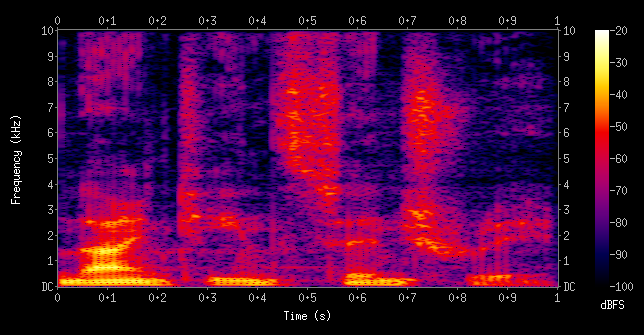
\includegraphics[width=0.7\textwidth]{img/Spectrogram-19thC.png} 
\end{frame}

\begin{frame}[t]{음성학의 하위 분야}
    \begin{block}{청취음성학(auditory phonetics)}
        귀로 소리를 듣고 음성으로 파악하는 과정 연구 (신경의학, 의학, 언어병리학 연계)
    \end{block}
    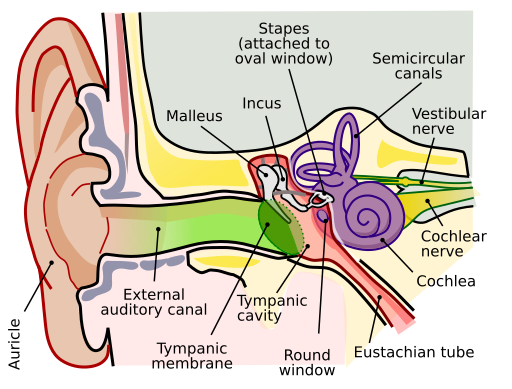
\includegraphics[width=0.5\textwidth]{img/Anatomy_of_the_Human_Ear.png}
\end{frame}

\section{발음 기관}

\begin{frame}[t]{발동부, 발성부, 조음부}
    \begin{columns}
        \begin{column}[T]{0.43\textwidth}
            \begin{block}{발동부}
                공기의 흐름을 만드는 기관
            \end{block}
            \begin{block}{발성부}
                소리의 울림과 높낮이를 결정하는 기관
            \end{block}
            \begin{block}{조음부}
                소리의 특징을 빚어내는 기관
            \end{block}
        \end{column}
        \begin{column}[T]{0.5\textwidth}
            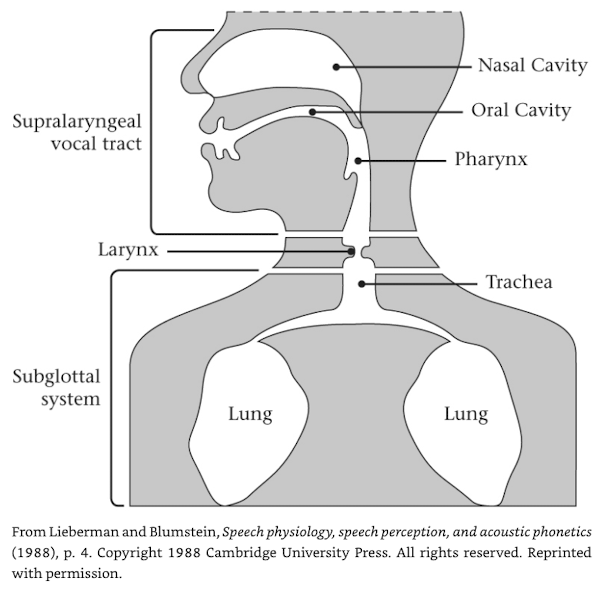
\includegraphics[height=0.8\textheight]{img/speech_production_mechanism.png}
        \end{column}
    \end{columns}
\end{frame}

\begin{frame}[t]{발동부}
    \begin{block}{폐 기류(pulmonic airstream)}
        \begin{itemize}
            \item \textbf{기관:} 폐(lungs)
            \item \textbf{원리:} 폐의 움직임을 통해 공기의 흐름을 만듦
            \item \textbf{방향에 따른 구분}
                \begin{itemize}
                    \item 날숨 기류 (Egressive): 공기를 밖으로 내보냄 \\ \rightarrow 말소리를 만드는 가장 보편적인 방식
                    \item 들숨 기류 (Ingressive): 공기를 안으로 들여보냄 \\ \rightarrow 말소리를 만들 때 쓰이는 경우는 거의 없음
                \end{itemize}
            \item \textbf{특징:} 호흡에 얹혀가는 방식이라 효율적이고, 공기의 양과 속도를 제어하기 쉬움
        \end{itemize}
    \end{block}
    참조: 국제음성기호 차트의 Consonants(Pulmonic) 파트
\end{frame}

\begin{frame}[t]{발동부}
    \begin{block}{성문 기류(glottalic airstream)}
        \begin{itemize}
            \item \textbf{기관:} 성문(glottis)
            \item \textbf{원리:} 닫힌 성문을 피스톤처럼 위아래로 움직여 공기 압축/희박화
            \item 방출음(ejectives), 내파음(implosives) 등 특수한 자음 생성
        \end{itemize}
    \end{block}
    참조: 국제음성기호 차트의 Consonants(Non-pulmonic) 파트
    \begin{columns}
        \begin{column}[T]{0.46\textwidth}
            \begin{block}{방출음(ejectives)}
                \begin{itemize}
                    \item 성문 날숨 기류를 이용해 내는 소리
                    \item \textds{[’]} 구별 기호를 덧붙여 표기
                    \item \emoji{television} \href{https://youtu.be/rP0-MfE4zbA}{\underline{영어의 수의적 \textds{[k’]}}}
                \end{itemize}
            \end{block}           
        \end{column}
        \begin{column}[T]{0.47\textwidth}
            \begin{block}{내파음(implosives)}
                \begin{itemize}
                    \item 성문 들숨 기류를 이용해 내는 소리
                    \item 기호 위쪽에 오른쪽으로 꺾인 갈고리를 부착해서 표기 \textds{[ɓ, ɗ, ɠ]}
                    \item \emoji{speaker-low-volume} \href{https://www.phonetics.ucla.edu/course/chapter6/sindhi/sinhi.html}{\underline{Sindhi 어의 내파음}}
                \end{itemize}
            \end{block}                       
        \end{column}
    \end{columns}
\end{frame}

\begin{frame}[t]{발동부}
    \begin{block}{연구개 기류(Velaric Airstream)}
        \begin{itemize}
            \item \textbf{기관:} 혀와 연구개(tongue, velum)
            \item \textbf{원리:} 혀와 연구개로 입안에 진공 상태를 만들어 공기를 안으로 빨아들임
            \item 흡착음(clicks) 등 특수한 자음 생성
        \end{itemize}
    \end{block}
    참조: 국제음성기호 차트의 Consonants(Non-pulmonic) 파트
    \begin{block}{흡착음(clicks)}
        \begin{itemize}
            \item 연구개 들숨 기류를 이용해 내는 소리
            \item 조음 위치에 따라 \textds{[ʘ] [ǀ] [ǁ] [ǂ] [ǃ]} 등의 기호를 붙여서 표시
            \item \emoji{speaker-low-volume} \href{https://www.phonetics.ucla.edu/course/chapter6/zulu/zulu.html}{\underline{줄루어의 흡착음}}
        \end{itemize}
    \end{block}
\end{frame}

\begin{frame}[t]{발성부}
    \begin{columns}
        \begin{column}[T]{0.5\textwidth}
            \begin{block}{성대(vocal cords)}
                \begin{itemize}
                    \item 후두에 있는 한 쌍의 근육
                    \item 열어두거나, 밀착시키거나, 좁힐 수 있음
                    \item 모양을 길게 늘리거나 짧게 줄일 수 있음
                \end{itemize}
            \end{block}
            \begin{block}{성문}
                성대 근육 사이의 공간
            \end{block}
        \end{column}
        \begin{column}[T]{0.43\textwidth}
            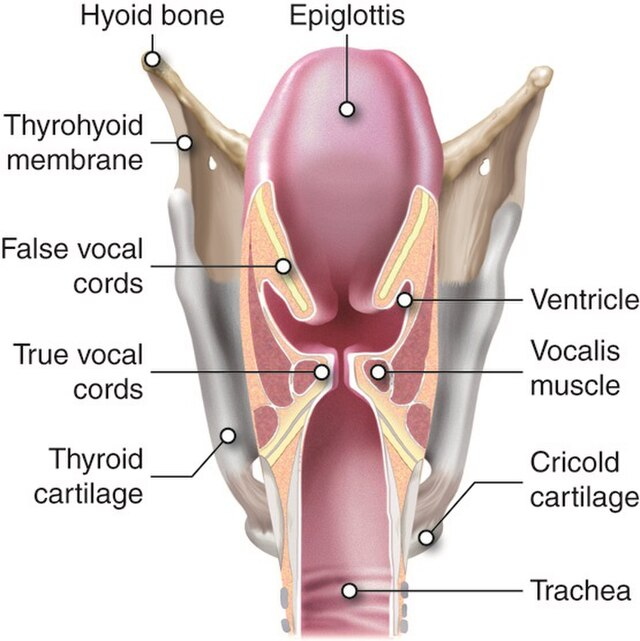
\includegraphics[width=1.0\textwidth]{img/Anatomytool_larynx_and_vocal_cords_English.jpg}
        \end{column}
    \end{columns}
\end{frame}

\begin{frame}[t]{발성부}
    \begin{columns}
        \begin{column}{0.5\textwidth}
            \begin{block}{무성음(voiceless)}
                성대 근육 열기 \rightarrow 성문 개방 \rightarrow 울림 없는 소리
            \end{block}
            \begin{block}{유성음(voiced)}
                성대 근육 밀착 \rightarrow 성문 개폐 빠르게 반복 \rightarrow 성대 진동 \rightarrow 울림을 동반하는 소리
            \end{block}
            {\small 실습: 입술을 부르르르르 떨어보세요!}
            \begin{block}{속삭임 소리}
                성대 근육 좁히기 \rightarrow 성문 반만 개방 \rightarrow 울림은 없으나 마찰음을 동반하는 소리
            \end{block}
        \end{column}
        \begin{column}{0.43\textwidth}
            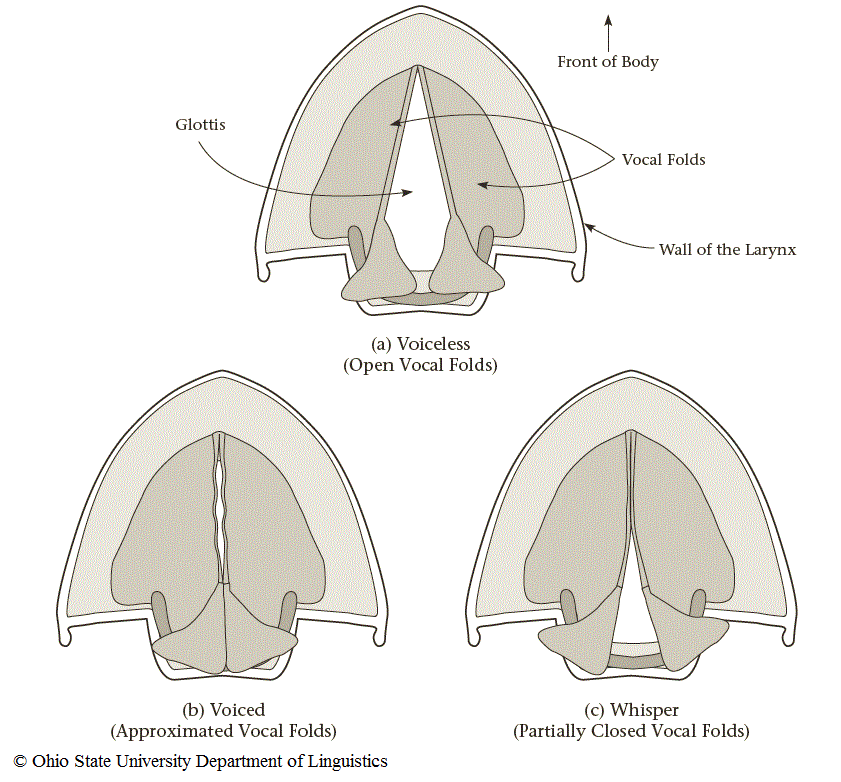
\includegraphics[width=1.0\textwidth]{img/VocalFolds.png}\\
            소리의 종류에 따른 성대의 모양
        \end{column}
    \end{columns}
\end{frame}

\begin{frame}[t]{}
    \begin{block}{높낮이}
        성대의 모양과 긴장 상태를 조절하여 소리의 기본 주파수를 바꿀 수 있음
    \end{block}
    \centering
    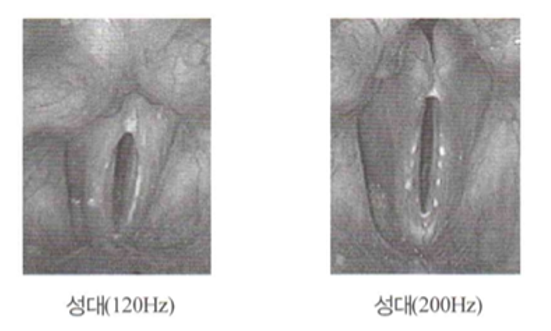
\includegraphics[width=0.7\textwidth]{img/vocal_folds_high_and_low_pitch.png}\\소리 높이에 따른 성대의 모양(좌: 낮은 소리, 우: 높은 소리) \\ 
    \small {강범모 (2020) 《언어:풀어쓴 언어학 개론》}   
\end{frame}

\begin{frame}[t]{조음부}
    \begin{block}{분절음(segments)}
        발성부를 거친 소리를 이용해서 만들어지는, 나뉘어져서 인식되는 소리
        \begin{itemize}
            \item 자음(consonants): 공기의 흐름이 막히거나 방해받아서 나는 소리
            \item 모음(vowels): 공기의 흐름이 막하지 않고 흐를 때 나는 소리
        \end{itemize}
    \end{block}
    \begin{block}{참고: 초분절음(suprasegments)}
        여러 분절음에 걸쳐서 부여되는 소리의 특성. 발동부, 발성부, 조음부의 협업으로 결정됨
        \begin{itemize}
            \item 강세: 크기(loudness). 폐가 내보내는 공기의 압력으로 결정
            \item 성조, 액센트, 억양: 높낮이(pitch). 성대의 진동 속도를 조절하여 결정
            \item 음장: 길이(duration). 발동부의 공기 공급과 조음부의 상태 유지 시간에 따라 결정
        \end{itemize}
    \end{block}
\end{frame}

\begin{frame}[t]{조음부}
    \begin{block}{자음의 분류}
        \begin{itemize}
            \item 조음 위치: 공기의 흐름이 어디에서 방해받는가? 
            \item 조음 방법: 공기의 흐름이 어떻게 방해받는가?
        \end{itemize}
    \end{block}
    \emoji{television} \href{https://seeingspeech.ac.uk}{\underline{분류별 자음의 조음 과정 살펴보기}}
\end{frame}

\begin{frame}[t]{조음부: 조음 위치에 따른 자음의 분류}
    \centering
    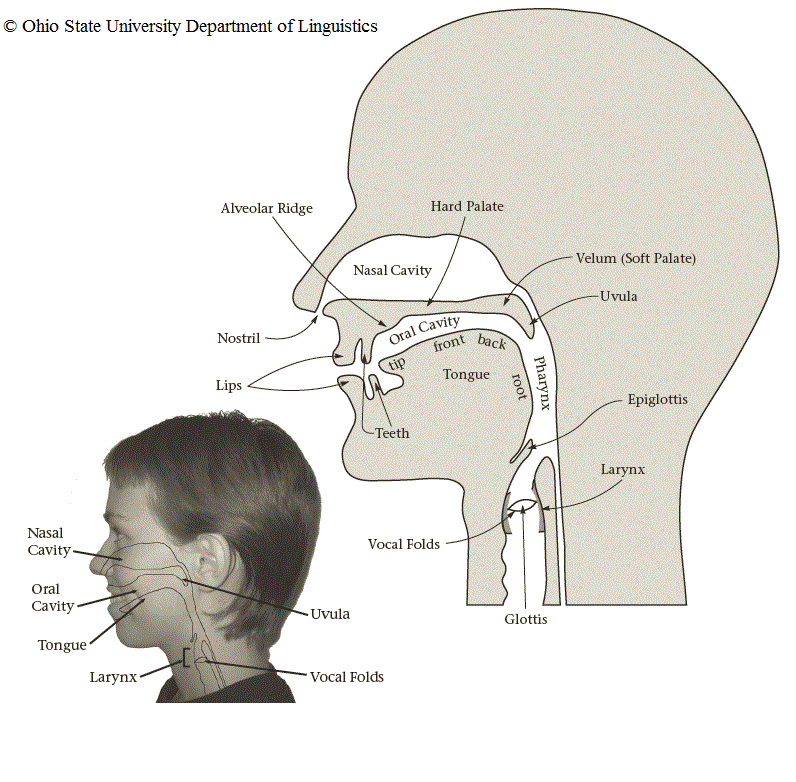
\includegraphics[height=1.0\textheight]{img/Saggital.png}
\end{frame}

\begin{frame}[t]{조음부: 조음 위치에 따른 자음의 분류}
    \begin{block}{양순음(bilabial)}
        \begin{itemize}
            \item 
            \item 
            \item 
        \end{itemize}
    \end{block}
    \begin{block}{순치음(labiodental)}
        \begin{itemize}
            \item 
            \item 
            \item 
        \end{itemize}
    \end{block}

\end{frame}

\begin{frame}[t]{조음부: 조음 위치에 따른 자음의 분류}
    \begin{block}{치음(dental)}
        \begin{itemize}
            \item 
            \item 
            \item 
        \end{itemize}
    \end{block}
    \begin{block}{치경음/치조음(alveolar)}
        \begin{itemize}
            \item 
            \item 
            \item 
        \end{itemize}
    \end{block}

\end{frame}

\begin{frame}[t]{조음부: 조음 위치에 따른 자음의 분류}
    \begin{block}{치경경구개음(postalveolar)}
        \begin{itemize}
            \item 
            \item 
            \item 
        \end{itemize}
    \end{block}
    \begin{block}{권설음(retroflex)}
        \begin{itemize}
            \item 
            \item 
            \item 
        \end{itemize}
    \end{block}

\end{frame}

\begin{frame}[t]{조음부: 조음 위치에 따른 자음의 분류}
    \begin{block}{경구개음(palatal)}
        \begin{itemize}
            \item 
            \item 
            \item 
        \end{itemize}
    \end{block}
    \begin{block}{연구개음(velar)}
        \begin{itemize}
            \item 
            \item 
            \item 
        \end{itemize}
    \end{block}

\end{frame}

\begin{frame}[t]{조음부: 조음 위치에 따른 자음의 분류}
    \begin{block}{구개수음(uvular)}
        \begin{itemize}
            \item 
            \item 
        \end{itemize}
    \end{block}
    \begin{block}{인두음(pharyngeal)}
        \begin{itemize}
            \item 
            \item 
        \end{itemize}
    \end{block}
    \begin{block}{성문음(glottal)}
        \begin{itemize}
            \item 
            \item 
        \end{itemize}
    \end{block}

\end{frame}


\begin{frame}[t]{조음부: 조음 방법에 따른 자음의 분류}
    \begin{block}{파열음(plosive)}
        \begin{itemize}
            \item 조음기관끼리 닿아서 공기의 흐름을 차단했다가 터뜨려 내는 소리
            \item 한국어 ㅂ \textds{[p]}, ㅍ \textds{[pʰ]}, ㅃ \textds{[p\textsuperscript{*}]}, ㄷ \textds{[t]}, ㅌ \textds{[tʰ]}, ㄸ \textds{[t\textsuperscript{*}]}, ㄱ \textds{[k]}, ㅋ \textds{[kʰ]}, ㄲ \textds{[k\textsuperscript{*}]}
            \item 영어 \textds{[p]}, \textds{[b]}, \textds{[t]}, \textds{[d]}, \textds{[k]}, \textds{[g]}
        \end{itemize}
    \end{block}
    \begin{block}{비음(nasal consonants)}
        \begin{itemize}
            \item 파열음과 같지만 입천장을 내려서 비강으로 통하는 공기길을 열어두고 내는 소리
            \item 한국어 ㅁ \textds{[m]}, ㄴ \textds{[n]}, 받침 ㅇ \textds{[ŋ]}
            \item 영어 \textds{[m]}, \textds{[n]}, \textds{[ŋ]}
        \end{itemize}
    \end{block}
\end{frame}

\begin{frame}[t]{조음부: 조음 방법에 따른 자음의 분류}
    \begin{block}{전동음(trill)}
        \begin{itemize}
            \item 조음기관을 떨면서 내는 소리
            \item \textds{[ʙ]}: 입술끼리 닿아서 떠는 소리
            \item \textds{[r]}: 혓날을 치경에 대고 떠는 소리
            \item \textds{[ʀ]}: 목젖을 혀의 뒷부분에 대고 떠는 소리
        \end{itemize}
    \end{block}
    \begin{block}{탄설음(tap/flap)}
        \begin{itemize}
            \item 혀를 치경 부분에 한번 탁 부딪혀 내는 소리
            \item 한국어의 음절초 ㄹ \textds{[ɾ]}
            \item 영국 영어의 어두 \textds{[ɾ]}
        \end{itemize}
    \end{block}

\end{frame}

\begin{frame}[t]{조음부: 조음 방법에 따른 자음의 분류}
    \begin{block}{}
        \begin{itemize}
            \item 
            \item 
            \item 
        \end{itemize}
    \end{block}
    \begin{block}{}
        \begin{itemize}
            \item 
            \item 
            \item 
        \end{itemize}
    \end{block}

\end{frame}





\end{document}